\documentclass{article}%
\usepackage[T1]{fontenc}%
\usepackage[utf8]{inputenc}%
\usepackage{lmodern}%
\usepackage{textcomp}%
\usepackage{lastpage}%
\usepackage[head=40pt,margin=0.5in,bottom=0.6in]{geometry}%
\usepackage{graphicx}%
%
\title{\textbf{Vecinos de Santa Elena en Mérida protestaron por falta de gas doméstico}}%
\author{El Nacional Web}%
\date{05/12/2018}%
%
\begin{document}%
\normalsize%
\maketitle%
\textbf{URL: }%
http://www.el{-}nacional.com/noticias/protestas/vecinos{-}santa{-}elena{-}merida{-}protestaron{-}por{-}falta{-}gas{-}domestico\_262200\newline%
%
\textbf{Periodico: }%
EN, %
ID: %
262200, %
Seccion: %
Protestas\newline%
%
\textbf{Palabras Claves: }%
NO\_TIENE\newline%
%
\textbf{Derecho: }%
2.8, %
Otros Derechos: %
, %
Sub Derechos: %
2.8.1\newline%
%
\textbf{EP: }%
SI\newline%
\newline%
%
\textbf{\textit{Los afectados salieron con pancartas a la calle para exigir respuesta por la falta de distribución}}%
\newline%
\newline%
%
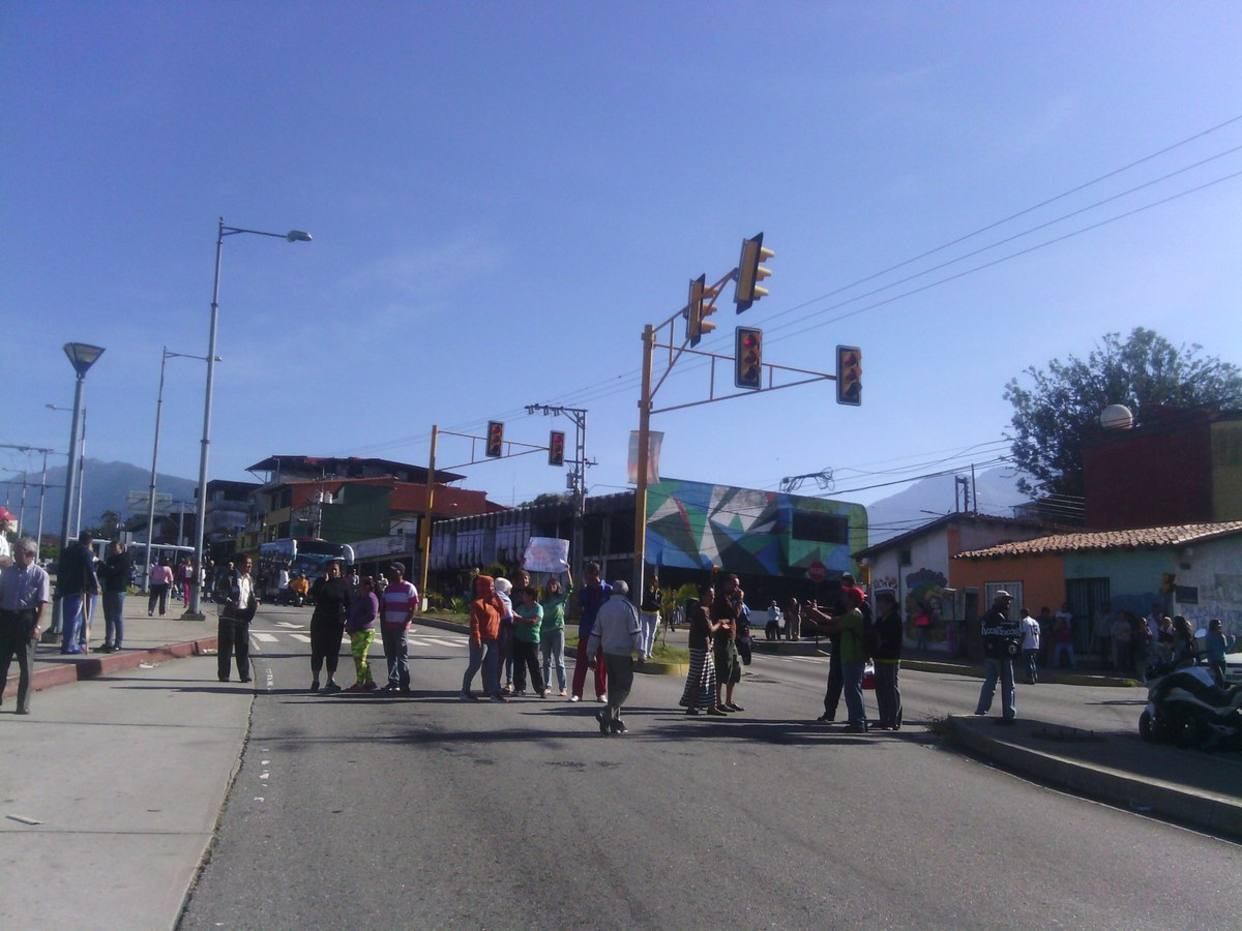
\includegraphics[width=300px]{4.jpg}%
\newline%
%
Vecinos de Santa Elena, estado Mérida, protestaron~este miércoles en la avenida 16 de septiembre por falta de gas doméstico. Desde las 9:15 am salieron a la calle con pancartas.%
\newline%
%
Reportes de Twitter indicaron~que el candidato a concejal en la localidad por el Partido Socialista Unido de Venezuela (PSUV)~entregará~a la 1:00 pm~las bombonas.%
\newline%
%
El martes 4 de diciembre también se registró una manifestación~en la plaza de Santa Elena para exigir respuesta por la falla de suministro de gas.%
\newline%
%
\end{document}